%!TEX root = ../../thesis.tex

\section{Deriving {RV} for synthetic spectra}
The work of this chapter extends the work of~\citep{figueira_radial_2016}.
To contrast the software improvements made here the details of~\citep{figueira_radial_2016} are first presented.
The important factors that were considered in preparing and using the synthetic spectra to apply the {RV} precision formulation of \cref{eqn:dv_rms,eqn:weighted_average_error}.

\subsection{Prepare {PHOENIX-ACES} models}
Four {PHOENIX-ACES} spectra were selected, spanning the M-dwarfs regime (M0, {M3}, {M6}, {M9}) with model temperatures 3900, 3500, 2800 and 2600\K{} respectively.
The other model parameters were \Logg=4.5, \feh{}=0 and \alphafe=0 representing values typical for M-dwarfs.
The flux (spectral energy distribution) given by the library spectra (\si{{ergs} \per\second\per\centi\meter\squared\per\centi\metre}) are converted into photon counts by dividing the flux by the energy of a photon, \({E}_{p}=hc/\lambda\).
Neglecting the multiplicative constants, this corresponds to multiplying the flux values by the respective wavelength.
In this case the absolute values do not matter, just the spectral shape, as the spectra will be scaled to a given \snr{} level.

\subsection{Convolution}
\label{subsec:convolutions}
To match realistic observations the spectra are convolved by a rotation kernel followed by a Gaussian instrumental kernel to broaden the spectra lines.
The details of these kernels and implementation of numerical convolution are given below.

\subsubsection*{Rotational convolution}
\label{subsubsec:rotational_convolution}
Stellar rotation has the affect of broadening spectral lines as the different portions of the stellar surface have a different radial velocity between \(\pm\)\Vsini{}.
Rotation is applied to a non-rotating spectrum by convolution with a rotation kernel.
The stellar rotational kernel used follows~\citet{gray_observation_2005};
\begin{align}
G(\Delta\lambda) &= \frac{2(1-\epsilon){[1-{(\Delta\lambda /{\Delta\lambda}_{L})}^{2}]}^{1/2} + \frac{1}{2}\pi\epsilon[1-{(\Delta\lambda /{\Delta\lambda}_{L})}^{2}]}{\pi (1-\epsilon/3) \vsini}\\
&= c_{1}{[1- {(\Delta\lambda /\Delta\lambda_{L})}^{2}]}^{1/2} + c_{2}[1-{(\Delta\lambda /\Delta\lambda_{L})}^{2}] \label{eqn:rotational_profile}
\end{align}
where
\begin{equation}
{c}_{1} = \frac{2(1-\epsilon)} {\pi (1-\epsilon/3)\vsini}, \hspace{4em} {c}_{2} = \frac{\frac{1}{2}\pi\epsilon} {\pi (1-\epsilon/3)\vsini},
\end{equation}
are constants which depend on the equatorial rotational velocity \Vsini{}.

Here $\Delta\lambda$ is the wavelength position from the non-rotating line centre, $\Delta\lambda_{L}$ is the maximum line shift of the line centre at the edge of the stellar disk where the Doppler shift is \Vsini{}; $\Delta\lambda_{L} = \lambda \frac{\vsini}{c}$.

This kernel arises from integrating the rotational velocity profile across the surface of the stellar disk as a series of strips with different Doppler shifts.
As such the rotation kernel is bounded in the range $[-\Delta\lambda_L, \Delta\lambda_{L}]$ from the line centre.
This can be seen in \cref{fig:rotationdiagram_and_profile} with a diagram of the stellar disk on the left, and the profile of the rotational kernel on the right, split into the two components from \cref{eqn:rotational_profile}.
This kernel also accounts for limb-darkening on the stellar disk with the linear limb darkening coefficient used in this work fixed at $\epsilon=0.6$ as done in~\citet{figueira_radial_2016}.

\begin{figure}
    \centering
    \begin{tabular}{cc}
        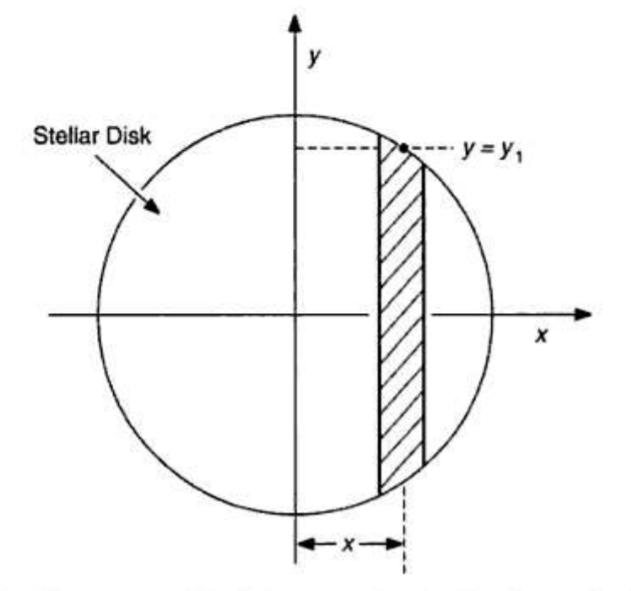
\includegraphics[width=0.45\linewidth]{figures/information-content/rotation_diagram} & 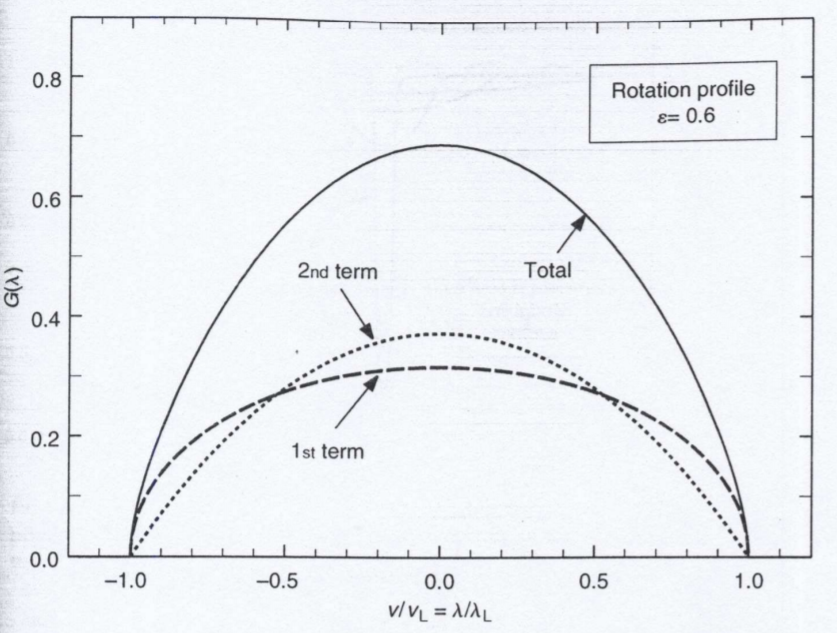
\includegraphics[width=0.45\linewidth]{figures/information-content/rotational_profile}\\
    \end{tabular}
    \caption{Left: Apparent disk of the star, thought of as a series of strips parallel to the projected rotation axis, each with the Doppler shift proportional to \(x\).
        The amount of light at each Doppler shift varies with the length of the strip, from \(-y_1\) to \(+y_1\), where \(y_1 = \sqrt{R^2-x^2}\) for a circular disk.
        Right: The rotation profile, \cref{eqn:rotational_profile}, is shown by the solid line black line for a limb darkening coefficient \(\epsilon=0.6\) and labelled ``total''.
        It is the sum of the ```1st term'' and ``2nd term'' curves.
        These are reproductions of Figures 18.3 and 18.5 from~\citep{gray_observation_2005}.}
    \label{fig:rotationdiagram_and_profile}
\end{figure}


As the Doppler shift \Vsini{} is transformed into wavelength by multiplication of $\lambda / c$ there is a wavelength dependence on the rotation kernel shape.
That is, the rotation kernel at each pixel is unique, requiring individual calculations.

\subsubsection*{Instrumental convolution}
\label{subsubsec:instrumental_convolution}
Following the rotational convolution the spectra are convolved with Gaussian instrumental profile ({\IP{}}) with the {\fwhm}  constrained by the given spectral resolution R, $\fwhm=\lambda/R$.

The Gaussian convolution kernel is of the form
\begin{equation}
IP(\Delta\lambda) = \frac{1}{\sigma \sqrt{2\pi}} \exp^{-\frac{{\Delta\lambda}^{2}}{2 {\sigma}^{2}}}
\label{eqn:IP_profile}
\end{equation}
with $\sigma = \frac{\fwhm}{2\sqrt{2 \ln(2)}}$, and $\Delta \lambda$ is again the difference from the line centre\footnote{Normally this is written as $(x-\mu)$ with $\mu$ as the Gaussian centre.}.

This assumes that the instrument profile of a particular instrument is in-fact Gaussian.
This assumption of a Gaussian instrumental profile is a good starting point for high-resolution spectrographs, and shown to be valid for CRIRES~\citep{seifahrt_synthesising_2010}.
If a non-Gaussian instrument profile is particularly well characterized, then it could be used to replace the Gaussian profile used here.

For instance~\citet{artigau_optical_2018} state that the instrumental profile of a (circular) fibre-fed spectrograph such as {HARPS} is mathematically equivalent to a cosine between $-\frac{\pi}{2}$ and $\frac{\pi}{2}$ with a width equivalent to the Gaussian {\fwhm}.
From this description the integration of a circular fibre is given by
\begin{equation}
\IP{}_{\textrm{fibre}(\Delta\lambda)} = \cos(B\cdot\Delta\lambda),  \hspace{2em} [-\frac{\pi}{2 B}, \frac{\pi}{2 B}],
\end{equation}
where {$B = \frac{\fwhm_{0}}{\fwhm}$ } is scaled to give the same area.
\citet{artigau_optical_2018} also mention that the {RV} precision results using this $\IP{}_{\textrm{fibre}}$ are all consistent with the results from a Gaussian kernel.
It only provides a small correction to the Gaussian profile of a standard spectrograph, and only necessary if one is resolution-limited by the slit.% (priv.\ comm. Pedro Figueira)

\subsubsection*{Numerical Convolution}
\label{subsubsec:numerical_convolution}
\todo{I think you should describe what is a numerical convolution before you describe the different types of numerical convolutions.}
Both convolutions are performed numerically, by iterating over all pixels in the spectrum.
At each pixel, a window of neighbouring pixels is selected that fall within the convolution window\footnote{Region in which the convolution kernel will affect this particular pixel.}, e.g.\ \(5\times\)\fwhm{} for that pixel.
The convolution kernel is calculated for the window, multiplied by the spectral flux and then summed to produce the new value for the pixel of the iteration.
The shape of the convolution kernels and the size of convolution window are wavelength dependant (\(\Delta\lambda_{L}=\lambda \frac{\vsini}{c}\) and \({\fwhm}=\frac{\lambda}{R}\)) and must be calculated separately for each pixel, making the convolution computationally expensive.

This convolution method allows for the spectrum to be non-uniformly spaced, unlike other methods that usually require uniform spacing e.g.\ the implementation in \pyastronomy{}.
One factor the needs consideration when convolving with an non-uniformly spaced spectrum is the discretization\todo{duplicated} of the kernel onto the wavelength grid.
For instance the number of points inside the convolution window, due to the sampling, as well as their specific location inside the kernel will have a slightly affect the kernel area.
The convolution result is normalized by dividing it by the result of the convolution kernel applied to a unitary spectrum of ones on the same wavelength grid.
\citet{figueira_radial_2016} performed this unitary convolution separately and applied the normalization correction afterwards.
In the improved implementation of \cref{sec:eniric} the convolution normalization is performed inside the loop over the pixels, directly for each pixel following the convolution calculation result for that pixel.

One factor the needs consideration when convolving with an non-uniformly spaced spectrum is the discretization of the kernel onto the wavelength grid.
For instance the number of points inside the convolution window, due to the sampling, as well as their specific location inside the kernel will have a slightly affect the kernel area.
The convolution result is normalized by dividing it by the result of the convolution kernel applied to a unitary spectrum of ones on the same wavelength grid.
\citet{figueira_radial_2016} performed this unitary convolution separately and applied the normalization correction afterwards.
In the improved implementation of \cref{sec:eniric} the convolution normalization is performed inside the loop over the pixels, directly for each pixel following the convolution calculation result for that pixel.

\todo{repeated}By default edge effects, in which pixels near the ends are not symmetrically convolved, are avoided on the spectral range desired by providing an input spectra that is sufficiently wider than the desired output spectrum.
Since two convolutions are performed one after the other the original input spectrum is selected to be wide enough such that no edge effects will be present in final output spectrum after both convolutions.\todo{be clearer}

\subsection{Interpolation}
\label{subsec:orginal_interpolation}
To simulate the sampling effect of high-resolution spectrographs interpolation is used to re-sample the spectrum to three pixels per resolution element.
This corresponds to a spacing between pixel at \(\lambda\) of (\(\lambda / 3R\)).
For echelle spectrographs, for which \(\Delta\lambda/\lambda\) is constant, the number of pixels per resolution element is also constant.
A sampling of three is chosen to be above the Nyquist limit of two pixels per resolution element, to not lose any spectral information, and commonly achieved by current spectrographs, e.g.\ a sampling of 3.3 for HARPS~\citep{mayor_setting_2003}.
This interpolation of the synthetic spectra is performed after the convolution and before the \snr scaling below.

\subsection{\snr{} scaling}
\label{subsec:orginal_snr_scaling}
The purpose of~\citet{figueira_radial_2016} was to compute only the relative precisions between the synthetic models.
This was done by normalizing each spectrum, after convolution, to a \snr{} of 100 at the centre of the \emph{J}-band.
Specifically this is achieved by summing the number pixels within one resolution element (three in this case), governed by the sampling, centred at 1.25\um{} and scaling the result so that the sum becomes \(100^2\).
In this way the \(\snr{} =\sqrt{F}\) is 100, where \(F\) is the sum of the three pixels.
The specific scaling values for the analysed spectra, \Vsini{}, and resolution combinations were hard coded into the software, making it impossible analyse a new spectrum without modification of the source code.

\subsection{Bands}
\label{subsec:orginal_bands}
To analyse the precision in different wavelength bands the spectra are split into several chunks.
The bands studied are the \emph{Z}, \emph{Y}, \emph{J}, \emph{H}, \emph{K}-bands with the specific wavelength bounds given in \cref{tab:infrared_bands}.
These are the \nir{} wavelength bands created by regions of strong water absorption in the Earth atmosphere.
These strong \ce{H2O} regions that defined these bands can be seen in the telluric spectrum given in \cref{fig:croppedmolecfitabsorbtion} or in the raw {CARMENES} spectra in \cref{fig:carmenes_raw} Figure~\reference{Add figure here}\todo{Add figure here}.

\subsection{Precision calculations}
\label{subsec:orginal_rv_calc}
Finally the computation of the {RV} precision application of \cref{eqn:dv_rms} is applied to the individual convolved spectra, normalized, and split into separate bands.
The {RV} precision calculations were performed under three separate conditions to assess different telluric line treatments.
The same three conditions are explored in this work, and to avoid repetition these conditions are detailed below in \cref{subsec:masking_function}.
